\documentclass[10pt,a4paper]{article}
\usepackage[a4paper]{geometry}

\usepackage[utf8x]{inputenc}
\usepackage{polski}

\usepackage{amsmath}
\usepackage{amssymb}
\usepackage{amsthm}

\usepackage{graphicx}
\usepackage{sidecap}

\theoremstyle{plain}
\newtheorem{theorem}{Twierdzenie}
\newtheorem{lemma}{Lemat}
\theoremstyle{definition}
\newtheorem*{definition}{Definicja}
\newtheorem*{example}{Przykład}
\newtheorem*{remark}{Uwaga}

\newcommand{\impl}{\rightarrow}
\newcommand{\N}{\mathbb{N}}

\newcommand{\header}[1]{\noindent\textbf{#1}}

\title{Teoria Programowanie w Logice}
\author{}
\date{Semestr letni 2013}

\begin{document}
\maketitle

\section{Dowody Hilberta i twierdzenie Posta o pełności}

\header{Język:}

\begin{itemize}
  \item przeliczalnie wiele zmiennych: $\{x_i\}_{i\in\N}$;
  \item funktory: $\impl, \neg$;
  \item zbiór formuł sensownych $S$: najmniejszy zbiór, taki że:
  \begin{enumerate}
    \item $\{x_i\} \subset S$;
    \item jeśli $A, B \in S$, to $A \impl B \in S$ i $\neg A \in S$.
  \end{enumerate}
\end{itemize}

\begin{definition}
$D \subset S$ jest zamknięty na Modus Ponens (MP), gdy
$$\text{jeśli } A \impl B \in D \text{ i } A \in D \text{, to } B \in D.$$
\end{definition}

\begin{lemma}
Jeśli $\alpha$ to pewna rodzina zbiorów zamkniętych na MP,
to $\bigcap\alpha$ jest zamknięty na MP.
\end{lemma}

\begin{lemma}
Jeśli $\alpha$ to pewna rodzina zbiorów zamkniętych na MP, która jest łańcuchem,
to $\bigcup\alpha$ jest zamknięty na MP.
\end{lemma}

\begin{lemma}
Dla każdego $X \subset S$ istnieje najmniejszy zbiór $Y$, taki że
\begin{enumerate}
  \item $X \subset Y$;
  \item $Y$ jest zamknięty na MP.
\end{enumerate}
\end{lemma}

\begin{proof}
$Y = \bigcap \{
  Z \subset S : X \subset Z \text{ i } Z \text { zamknięty na MP}
\}.$
\end{proof}

Taki $Y$ nazywamy \emph{konsekwencją} $X$. ($Cn: 2^S \ni X \mapsto Y \in 2^S$)

\bigskip

\header{Fakty o $Cn$}

\begin{enumerate}
  \item Jeśli $X$ jest zamknięty na MP, to $Cn(X) = X$.
  \item $X \subset Cn(X)$.
  \item Jeśli $X \subset Y$, to $Cn(X) \subset Cn(Y)$.
  \item $Cn(Cn(X)) = Cn(X)$.
  \item $Cn(X) = \bigcup\{
    Cn(Y) : Y \subset X \text{ i } X \text{ jest skończony}
  \}$.
    \begin{proof}
      $\supset$ -- trywialny. $\subset$ -- Wystarczy pokazać, że prawa strona
      jest zamknięta na MP. $A \impl B \in \bigcup \{ \ldots \}$, więc
      $A \impl B \in Cn(Y_1)$, $A \in \bigcup \{ \ldots \}$, więc
      $A \in Cn(Y_2)$, zatem $B \in Cn(Y_1 \cup Y_2)$.
      Na koniec zauważamy, że $Y_1 \cup Y_2$ jest skończonym podzbiorem $X$.
    \end{proof}
  \item $Cn(\emptyset) = \emptyset$.
\end{enumerate}

\bigskip

\header{Alternatywne opisy $Cn$}
\begin{align*}
& H^i: 2^S \to 2^S\\
& H^0(X) = X\\
& H^{n+1}(X) = H^n(X) \cup \{
    B \in S : \exists_{A \in S} (A \impl B \in H^n(X) \text{ i } A \in H^n(X))
  \}\\
& H(X) = \bigcup_{n = 0}^\infty H^n(X)
\end{align*}

\begin{lemma}
$Cn(X) = H(X).$
\end{lemma}

\begin{proof}
$\subset$ -- łatwy, $\supset$ -- przez indukcję ze względu na $n$.
\end{proof}

\begin{definition}[Dowód Hilberta]
$A \in S$ ma dowód Hilberta ze zbioru formuł $X$, gdy istnieje skończony ciąg
formuł $A_0, A_1, \ldots, A_n$, taki że $A_n = A$ i dla każdego $i$:
\begin{itemize}
  \item $A_i \in X$ lub
  \item istnieją $A_j, A_k$, takie że $j, k < i$ i $A_j = A_k \impl A_i$.
\end{itemize}
\end{definition}

%TODO: tu by można jeszcze wspomnieć o drzewowej reprezentacji dowodu.

\begin{definition}[Konsewkencja dowodowa]
$Cn^*(X) := \{ A \in S: A \text{ ma dowód z } X\}$
\end{definition}

\begin{lemma}
$Cn(X) = Cn^*(X)$
\end{lemma}

\begin{proof}
$\supset$ -- przez indukcję ze względu na długość dowodu,
$\subset$ -- przez sklejenie dowodów Hilberta.
%TODO: tę drugą część można by rozpisać dokładniej.
\end{proof}

\bigskip

\begin{definition}[Logika klasyczna]
Niech $L \subset S$ będzie najmniejszym zbiorem zawierającym (dla dowolnych
$A, B, C \in S$)
\begin{itemize}
  \item $K: A \impl (B \impl A)$
  \item $S: (A \impl (B \impl C)) \impl ((A \impl B) \impl (A \impl C))$
  \item $N: (\neg A \impl \neg B) \impl ((\neg A \impl B) \impl A)$
\end{itemize}
oraz zamkniętym na MP.
\end{definition}

\begin{example}
$I: A \impl A \in L$, ponieważ:
\begin{itemize}
  \item $(A \impl (B \impl A)) \impl ((A \impl B) \impl (A \impl A))$
    \quad(aksjomat $S$)
  \item $A \impl (B \impl A)$ \quad(aksjomat $K$)
  \item $(A \impl B) \impl (A \impl A)$ \quad(Modus Ponens)
  \item $(A \impl (C \impl A)) \impl (A \impl A)$ \quad($B := C \impl A$)
  \item $A \impl (C \impl A)$ \quad(aksjomat $K$)
  \item $A \impl A$ \quad(Modus Ponens)
\end{itemize}
\end{example}

\noindent Notacja: $Cn_L(X) := C_n(L \cup X)$.

\begin{theorem}[O dedukcji wprost, TDW]
$b \in Cn_L(X \cup \{a\})$ wtedy i tylko wtedy, gdy $a \impl b \in Cn_L(X)$.
\end{theorem}

\begin{proof}
$\Leftarrow$ -- trywialny. $\Rightarrow$ -- przez indukcję ze względu
na długość dowodu $b$.  %TODO: napisać tę drugą część.
\end{proof}

\begin{theorem}[O dedukcji nie wprost, TDN]
Jeśli $z, \neg z \in Cn_L(X \cup \{a, \neg b\})$, to $a \impl b \in Cn_L(X)$.
\end{theorem}

\begin{proof}
\begin{flalign*}
\neg b \impl z &\in Cn_L(X \cup \{a\}) && \text{z TDW}\\
\neg b \impl \neg z &\in Cn_L(X \cup \{a\}) && \text{z TDW}\\
(\neg b \impl \neg z) \impl ((\neg b \impl z) \impl b) 
  &\in L \subset Cn_L(X \cup\{a\}) && \text{aksjomat N}\\
b &\in Cn_L(X \cup \{a\}) && \text{MP} \times 2\\
a \impl b &\in Cn_L(X) && \text{TDW}
\end{flalign*}
\end{proof}

\begin{theorem}
Jeśli $L' \subset S$ jest zbiorem zamkniętym na MP, w którym prawdziwe jest TDW,
to $K, S \in L'$.
\end{theorem}

\begin{proof}
 ~\begin{itemize}
    \item $K \in L'$:
      \begin{flalign*}
        a &\in Cn_{L'}(\{a\} \cup \{b\}) && \\
        b \impl a &\in Cn_{L'}(\{a\}) && \text{z TDW} \\
        a \impl (b \impl a) &\in Cn_{L'}(\emptyset) = L' && \text{z TDW}
      \end{flalign*}
    \item $S \in L'$:
      \begin{flalign*}
        a &\in Cn_{L'}(\{a\impl (b\impl c), a \impl b, a\}) && \\
        b &\in Cn_{L'}(\{a\impl (b\impl c), a \impl b, a\}) &&
        \text{MP na }a\impl b\text{ i }a \\
        b \impl c &\in Cn_{L'}(\{a\impl (b\impl c), a \impl b, a\}) &&
        \text{MP na }a\impl (b \impl c)\text{ i }a \\
        c &\in Cn_{L'}(\{a\impl (b\impl c), a \impl b, a\}) &&
        \text{MP na }b \impl c\text{ i }b \\
        (a \impl c) &\in Cn_{L'}(\{a\impl (b\impl c), a \impl b\}) &&
        \text{z TDW} \\
        (a\impl b) \impl (a \impl c) &\in Cn_{L'}(\{a\impl (b\impl c)\}) &&
        \text{z TDW} \\
        (a\impl (b\impl c)) \impl ((a\impl b) \impl (a \impl c)) &\in
        Cn_{L'}(\emptyset) = L' && \text{z TDW} 
      \end{flalign*}
  \end{itemize}
\end{proof}

\begin{theorem}
Jeśli $L' \subset S$ jest zbiorem zamkniętym na MP, w którym prawdziwe jest TDN,
to $K, S, N \in L'$.
\end{theorem}

\begin{proof}
  ~\begin{itemize}
    \item W~$L'$ zachodzi TDW (zatem $K, S \in L'$):
      \begin{itemize}
        \item W każdym zbiorze zamkniętym na MP zachodzi:
          jeśli $b \impl a \in Cn_{L'}(X)$, to $a \in Cn_{L'}(X\cup\{b\})$.
        \item Implikacja w drugą stronę (jeśli $a \in Cn_{L'}(X\cup\{b\})$,
            to $b \impl a \in Cn_{L'}(X)$) zachodzi, bo:
          \begin{flalign*}
            a &\in Cn_{L'}(X\cup\{b\}) \subset Cn_{L'}(X\cup\{b,\neg a\})
            && \text{z założenia} \\
            \neg a &\in Cn_{L'}(X\cup\{b,\neg a\}) && \\
            b \impl a &\in Cn_{L'}(X) && \text{z TDN}
          \end{flalign*}
      \end{itemize}
    \item $N \in L'$:
      \begin{flalign*}
        \neg b, b &\in Cn_{L'}(\{\neg a \impl \neg b,\neg a \impl b, \neg a\})
        && \text{dwa razy MP} \\
        (\neg a \impl b) \impl a &\in Cn_{L'}(\{\neg a \impl \neg b\})
        && \text{z TDN} \\
        (\neg a \impl \neg b) \impl ((\neg a \impl b) \impl a)
        &\in Cn_{L'}(\emptyset) && \text{z TDW}
      \end{flalign*}
  \end{itemize}
\end{proof}

\header{Konstrukcje drzewowe dowodów}

\begin{figure}[h]
\caption{Drzewo Modus Ponens}
\centering 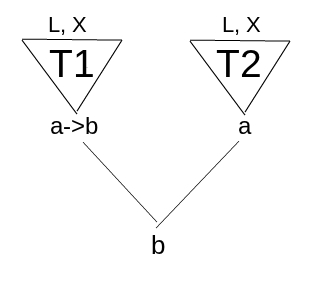
\includegraphics[width=0.3\textwidth]{img/drzewoMP}
\end{figure}

\begin{figure}[h]
\caption{TDW jako transformacja drzewa dowodu}
\centering 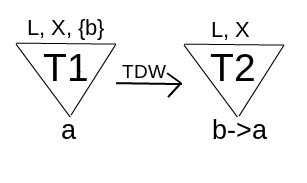
\includegraphics[width=0.4\textwidth]{img/drzewoTDW}
\end{figure}

Baza indukcji konstrukcji drzewa TDW:
\begin{itemize}
\item T1 jest punktem $a \in L \cup X$, robię $(K_{a, b}$ and $a) 
\Rightarrow b \rightarrow a$
\item T1 jest punktem $b$, robię $((S$ and $K)$ and $K) 
\Rightarrow b \rightarrow b$
\end{itemize}

\begin{figure}[h]
\caption{Indukcyjna konstrukcja drzewa TDW}
\centering 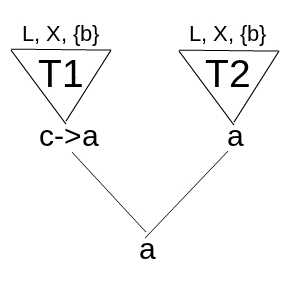
\includegraphics[width=0.25\textwidth]{img/drzewoMP2}
\centering 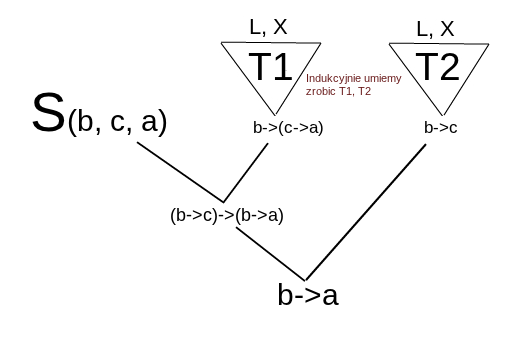
\includegraphics[width=0.5\textwidth]{img/drzewoTDWindukcyjnie}

\caption{Indukcyjna konstrukcja drzewa TDN}
\centering 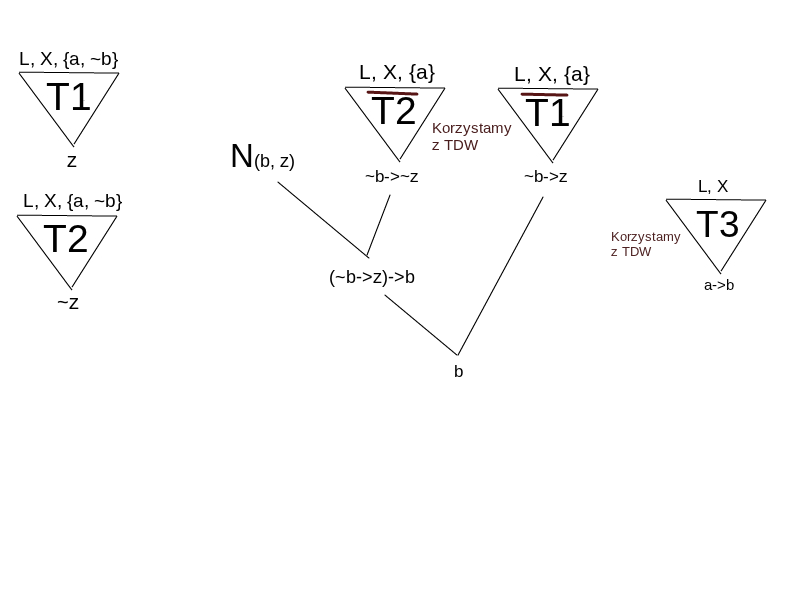
\includegraphics[width=0.7\textwidth]{img/drzewoTDN}
\end{figure}


\header{Ćwiczenia}

\begin{enumerate}
  \item $\neg \neg p \impl p \in L$.
      \quad Dowód: TDN dla $Cn_{L}(\{\neg \neg p, \neg p\})$.
  \item $p \impl \neg \neg p \in L$.
      \quad Dowód: 1. i TDN dla $Cn_{L}(\{p, \neg \neg \neg p\})$.
  \item $(p \impl q) \impl ((q \impl r) 
      \impl (p \impl r)) \in L$.
      \quad Dowód: TDW dla $Cn_{L}(\{p \impl q, q \impl r, p\})$.
  \item $(p \impl q) \impl (\neg q \impl \neg p) \in L$.
      \quad Dowód: TDN dla $Cn_{L}(\{p \impl q, \neg q, \neg \neg p\})$.
  \item Prawo wyłączonego środka:
      $(p \impl q) \impl ((\neg p \impl q) \impl q) \in L$.
    \begin{proof}
      \begin{flalign*}
        \neg q &\in Cn_{L}(\{p \impl q, \neg p \impl q, \neg q\}) &&\\
        \neg q \impl \neg p &\in Cn_{L}(\{p \impl q, \neg p \impl q, \neg q\})
            && \text{ćw. 4} \\
        \neg p &\in Cn_{L}(\{p \impl q, \neg p \impl q, \neg q\})
            && \text{MP} \\
        q &\in Cn_{L}(\{p \impl q, \neg p \impl q, \neg q\}) && \text{MP} \\
        (\neg p \impl q) \impl q &\in Cn_{L}(\{p \impl q\}) && \text{TDN} \\
        (p \impl q) \impl ((\neg p \impl q) \impl q) &\in Cn_{L}(\emptyset) = L
            && \text{TDW}
      \end{flalign*}
    \end{proof}
  \item Prawo Pierce'a: $((p \impl q) \impl p) \impl p \in L$.
    \begin{proof}
      \begin{flalign*}
        \neg p \impl (\neg q \impl \neg p) 
            &\in Cn_L(\{(p \impl q) \impl p, \neg p\}) && \text{aksjomat } S\\
        \neg q \impl \neg p &\in Cn_{L}(\cdots) && \text{MP}\\
        p \impl q &\in Cn_{L}(\cdots) && \text{ćw. 4}\\
        p &\in Cn_{L}(\cdots) && \text{MP}\\
        \neg p &\in Cn_{L}(\cdots) && \\
        ((p \impl q) \impl p) \impl p &\in Cn_{L}(\emptyset) = L && \text{TDN}
      \end{flalign*}
    \end{proof}
\end{enumerate}

\begin{remark}
  Pomimo że prawo Pierce'a da się wyrazić bez użycia negacji,
  \emph{nie należy ono} do logiki intuicjonistycznej (tzn.
  nie da się go wyprowadzić używając jedynie $K$ i~$S$).
\end{remark}

\begin{definition}
Zbiór $X \subset S$ jest sprzeczny, gdy $Cn_L(X) = S$.
\end{definition}

\begin{definition}
Zbiór $X \subset S$ jest zupełny, gdy 
$\forall_{a \in S} a \in S \text{ lub } \neg a \in S$.
\end{definition}

\begin{theorem}[Twierdzenie Lindenbauma]
Dowolny niesprzeczny zbiór $X \subset S$ może być rozszerzony do zbioru
$Y \supset X$, który jest zamknięty na MP, niesprzeczny i zupełny.
\end{theorem}

\begin{proof}[Dowód kreatywny]
Formuły to skończone napisy nad przeliczalnym alfabetem, zatem jest ich
przeliczalnie wiele. Możemy więc ustawić je w ciąg $s_0, s_1, \ldots$. 
Rozważmy ciąg $Y_i$, taki że $Y_0 = Cn_L(X)$ oraz

$$Y_{n+1} = \begin{cases}
  Cn_L(Y_n \cup \{s_n\}) & 
    \text{jeśli } Y_n \cup \{s_n\} \text{ jest niesprzeczny}\\
  Y_n & \text{wpp.}
\end{cases}$$

Niech $Y = \bigcup_{i\in\N} Y_i$. Wystarczy wykazać, że $Y$ ma własności
przedstawione w tezie.

Z definicji wynika, że zbiory $Y_i$ są zamknięte na MP, niesprzeczne 
i tworzą łańcuch. Łatwo można wykazać, że w takim razie również ich
suma jest zamknięta na MP i niesprzeczna.

Zupełność wymaga nieco więcej uwagi. Dowód przeprowadzimy nie wprost.
Załóżmy, że istnieje formuła $a$ taka, że $a, \neg a \not \in Y$.
Niech $a = s_i$ oraz $\neg a = s_j$. Skoro $a \not \in Y$, to
w szczególności $a \not \in Y_{i+1}$, zatem z definicji $Y_i \cup \{a\}$
jest sprzeczny. Analogicznie $Y_j \cup \{\neg a\}$ jest sprzeczny.
Oznaczmy $k=\max(i, j)$. Wtedy $Y_i,Y_j \subset Y_k$ i z monotoniczności
konsekwencji mamy, że $Cn_L(Y_k \cup \{a\}) = Cn_L(Y_k \cup \{\neg a\}) = S$.

Weźmy dowolną formułę $b \in S$. Z TDW mamy, że
$a \impl b, \neg a \impl b \in Cn_L(Y_k)$. Stosując prawo wyłączonego środka
możemy wykazać, że $b \in Y_k$. Skoro jednak $b$ było dowolną formułą, to
$Y_k = S$, co prowadzi do sprzeczności z faktem, że zbiory $Y_i$ są
niesprzeczne.
\end{proof}

\begin{proof}[Dowód bezmyślny]Z lematu Kuratowskiego-Zorna.\end{proof}

\begin{theorem}[Relatywne twierdzenie Lindenbauma]

Dla każdego zbioru $X \subset S$, takiego że $X = Cn_L(X)$, oraz każdej
formuły $a \not \in X$ istnieje zbiór $Y \subset S$, taki że
\begin{itemize}
  \item $Y \supset X$,
  \item $Y$ jest zamknięty na MP,
  \item $a \not \in Y$,
  \item $\forall_{b \not \in Y} a \in Cn_L(Y \cup \{b\})$ 
    ($Y$ nie da się już rozszerzyć zachowując powyższe warunki).
\end{itemize}
\end{theorem}

\begin{proof}Jak wyżej.\end{proof}

\begin{definition}
Matrycą logiczną nazywamy czwórkę $M=(U, U^*, f^\impl, f^\neg)$, taką że
\begin{itemize}
  \item $U \neq \emptyset$ -- wartości logiczne
  \item $\emptyset \neq U^* \subset U$ -- wartości wyróżnione (prawdziwe)
  \item $f^\impl : U^2 \to U$ -- ,,tabelka'' implikacji
  \item $f^\neg : U \to U$ -- ,,tabelka'' negacji
\end{itemize}
\end{definition}

\begin{definition}[Wartościowanie formuł w matrycy $M$]
$f : \{x_i\}_{i\in\N} \to U$ -- wartościowane zmiennych logicznych.
Istnieje (jedyne) rozszerzenie $f$ do $w^f : S \to U$, takie że
\begin{itemize}
  \item $w^f(x_i) = f(x_i)$,
  \item $w^f(A \impl B) = f^\impl(w^f(A), w^f(B))$,
  \item $w^f(\neg A) = f^\neg(w^f(A))$.
\end{itemize}
\end{definition}

\begin{definition}
$a \in S$ jest tautologią matrycy $M$, gdy $w^f(a) \in U^*$ dla dowolnego
wartościowania $f$.
\end{definition}

\begin{definition}
$E(M)$ -- zbiór wszystkich tautologii matrycy $M$.
\end{definition}

\begin{definition}
Reguła MP jest niezawodna w matrycy $M$, gdy
$$\forall_{x,y \in U}
  \text{ jeśli } x \in U^* \text{ i } f^\impl(x,y) \in U^*
  \text{ to } y \in U^*.$$
\end{definition}

\header{Obserwacja.} Jeśli MP jest niezawodna w $M$,
to $E(M)$ jest zamknięty na MP.

\bigskip

\header{Przykłady matryc logicznych:}

\begin{description}
  \item[Matryca Łukasiewicza]
    $U = \{1, 2, 3\}$, $U^* = \{3\}.$
    $$\begin{array}{r|lll}
      \impl & 1 & 2 & 3\\
      \hline
          1 & 3 & 3 & 3\\
          2 & 2 & 3 & 3\\
          3 & 1 & 2 & 3
    \end{array}\quad\begin{array}{r|l}
      \neg & \\
      \hline
         1 & 3\\
         2 & 2\\
         3 & 1
    \end{array}$$

  \item[Matryca Posta]
    $U = \{1, 2, 3\}$, $U^* = \{2, 3\}.$
    $$\begin{array}{r|lll}
      \impl & 1 & 2 & 3\\
      \hline
          1 & 3 & 3 & 3\\
          2 & 1 & 3 & 3\\
          3 & 1 & 2 & 3
    \end{array}\quad\begin{array}{r|l}
      \neg & \\
      \hline
         1 & 3\\
         2 & 2\\
         3 & 1
    \end{array}$$

  \item[Rodzina matryc $M_Z$]
    ($Z \neq \emptyset$ -- dowolny niepusty zbiór)
    \begin{align*}
      M_Z &= (U = 2^Z, U^* = \{Z\}, f^\impl, f^\neg),\\
      f^\impl (A, B) &= (Z \setminus A) \cup B,\\
      f^\neg (A) &= Z \setminus A.
    \end{align*}
\end{description}

\header{Obserwacje.} 

\begin{itemize}
  \item MP jest niezawodna we wszystkich powyższych matrycach.
  \item $K,S,N \in E(M_Z)$.
  \item $M_Z$ jest matrycą logiki klasycznej dla $Z$ takiego że $\#Z=1$.
\end{itemize}

\begin{definition}[Konsekwencja matrycowa]
$M$ -- matryca, w której MP jest niezawodna.
$$Cn^M(X) = \{ a \in S : \forall_f 
  ((\forall_{x \in X} w^f(x) \in U^*) \implies w^f(a) \in U^*) \}.$$
\end{definition}

\header{Fakty o $Cn^M$}

\begin{enumerate}
  \item $Cn^M(\emptyset) = E(M)$.
  \item $Cn^M(X)$ jest zamknięty na MP.
  \item $X \subset Cn^M(X)$.
  \item Jeśli $X \subset Y$, to $Cn^M(X) \subset Cn^M(Y)$.
  \item $Cn^M(Cn^M(X)) = Cn^M(X)$.
\end{enumerate}

\noindent Od teraz: $M$ -- matryca logiki klasycznej.

\begin{theorem}[O niesprzeczności]
$Cn_L(X) \subset Cn^M(X)$.
\end{theorem}

\begin{proof}
$L \subset E(M) = Cn^M(\emptyset) \subset Cn^M(X)$, $X \subset Cn^M(X)$
oraz $Cn^M(X)$ jest zamknięty na MP. Z drugiej strony
$Cn_L(X) = Cn(L \cup X)$ jest najmniejszym zbiorem spełniającym powyższe
trzy warunki, zatem inkluzja zachodzi.
\end{proof}

\begin{theorem}[O pełności Posta]
$Cn^M(X) \subset Cn_L(X)$.
\end{theorem}

%TODO: dowód pojawi się na kolejnym wykładzie.

\end{document}
